

% Gradient Info
  
\tikzset {_q6d1jly0c/.code = {\pgfsetadditionalshadetransform{ \pgftransformshift{\pgfpoint{-7.5 bp } { 0 bp }  }  \pgftransformrotate{-225 }  \pgftransformscale{2 }  }}}
\pgfdeclarehorizontalshading{_0bsmz13ng}{150bp}{rgb(0bp)=(0.03,0.22,0.4);
rgb(37.5bp)=(0.03,0.22,0.4);
rgb(62.5bp)=(0,0.29,0.51);
rgb(100bp)=(0,0.29,0.51)}

% Gradient Info
  
\tikzset {_uvoxzm524/.code = {\pgfsetadditionalshadetransform{ \pgftransformshift{\pgfpoint{-7.5 bp } { 0 bp }  }  \pgftransformrotate{-225 }  \pgftransformscale{2 }  }}}
\pgfdeclarehorizontalshading{_fyest5jbo}{150bp}{rgb(0bp)=(0.03,0.22,0.4);
rgb(37.5bp)=(0.03,0.22,0.4);
rgb(62.5bp)=(0,0.29,0.51);
rgb(100bp)=(0,0.29,0.51)}

% Gradient Info
  
\tikzset {_py27uv7b1/.code = {\pgfsetadditionalshadetransform{ \pgftransformshift{\pgfpoint{-7.5 bp } { 0 bp }  }  \pgftransformrotate{-225 }  \pgftransformscale{2 }  }}}
\pgfdeclarehorizontalshading{_e66njv4ua}{150bp}{rgb(0bp)=(0.03,0.22,0.4);
rgb(37.5bp)=(0.03,0.22,0.4);
rgb(62.5bp)=(0,0.29,0.51);
rgb(100bp)=(0,0.29,0.51)}
\tikzset{every picture/.style={line width=0.75pt}} %set default line width to 0.75pt        


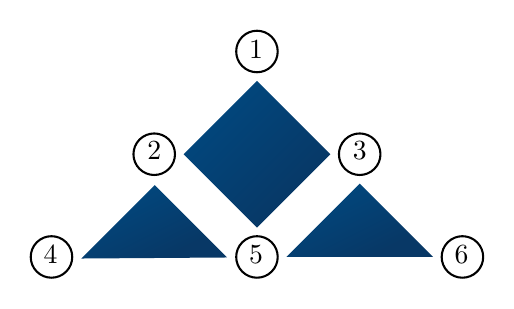
\begin{tikzpicture}[x=0.75pt,y=0.75pt,yscale=-1,xscale=1]
%uncomment if require: \path (0,141); %set diagram left start at 0, and has height of 141

%Shape: Square [id:dp40205531904810266] 
\draw  [draw opacity=0][shading=_0bsmz13ng,_q6d1jly0c] (120.31,35) -- (155.66,70.35) -- (120.31,105.71) -- (84.95,70.35) -- cycle ;
%Shape: Circle [id:dp6654608173556106] 
\draw   (113.24,13.78) .. controls (117.14,9.88) and (123.47,9.88) .. (127.38,13.78) .. controls (131.28,17.69) and (131.28,24.02) .. (127.38,27.92) .. controls (123.47,31.83) and (117.14,31.83) .. (113.24,27.92) .. controls (109.33,24.02) and (109.33,17.69) .. (113.24,13.78) -- cycle ;
%Shape: Circle [id:dp06811511385885272] 
\draw   (162.74,63.28) .. controls (166.64,59.37) and (172.97,59.37) .. (176.88,63.28) .. controls (180.78,67.19) and (180.78,73.52) .. (176.88,77.42) .. controls (172.97,81.33) and (166.64,81.33) .. (162.74,77.42) .. controls (158.83,73.52) and (158.83,67.19) .. (162.74,63.28) -- cycle ;
%Shape: Circle [id:dp866496050161264] 
\draw   (212.23,112.78) .. controls (216.14,108.87) and (222.47,108.87) .. (226.37,112.78) .. controls (230.28,116.68) and (230.28,123.01) .. (226.37,126.92) .. controls (222.47,130.82) and (216.14,130.82) .. (212.23,126.92) .. controls (208.33,123.01) and (208.33,116.68) .. (212.23,112.78) -- cycle ;
%Shape: Circle [id:dp8486257980974814] 
\draw   (63.74,63.28) .. controls (67.65,59.37) and (73.98,59.37) .. (77.88,63.28) .. controls (81.79,67.19) and (81.79,73.52) .. (77.88,77.42) .. controls (73.98,81.33) and (67.65,81.33) .. (63.74,77.42) .. controls (59.83,73.52) and (59.83,67.19) .. (63.74,63.28) -- cycle ;
%Shape: Circle [id:dp6621158362166136] 
\draw   (113.24,112.78) .. controls (117.14,108.87) and (123.47,108.87) .. (127.38,112.78) .. controls (131.28,116.68) and (131.28,123.01) .. (127.38,126.92) .. controls (123.47,130.82) and (117.14,130.82) .. (113.24,126.92) .. controls (109.33,123.01) and (109.33,116.68) .. (113.24,112.78) -- cycle ;
%Shape: Circle [id:dp9693194383410402] 
\draw   (14.24,112.78) .. controls (18.15,108.87) and (24.48,108.87) .. (28.38,112.78) .. controls (32.29,116.68) and (32.29,123.01) .. (28.38,126.92) .. controls (24.48,130.82) and (18.15,130.82) .. (14.24,126.92) .. controls (10.34,123.01) and (10.34,116.68) .. (14.24,112.78) -- cycle ;
%Shape: Right Triangle [id:dp28578880257729367] 
\draw  [draw opacity=0][shading=_fyest5jbo,_uvoxzm524] (105.92,120.1) -- (35.71,120.6) -- (71.06,85.24) -- cycle ;
%Shape: Right Triangle [id:dp9982201862645094] 
\draw  [draw opacity=0][shading=_e66njv4ua,_py27uv7b1] (205.16,119.85) -- (134.45,119.85) -- (169.81,84.49) -- cycle ;

% Text Node
\draw (115,14) node [anchor=north west][inner sep=0.75pt]   [align=left] {1};
% Text Node
\draw (66,63) node [anchor=north west][inner sep=0.75pt]   [align=left] {2};
% Text Node
\draw (165,63) node [anchor=north west][inner sep=0.75pt]   [align=left] {3};
% Text Node
\draw (16,113) node [anchor=north west][inner sep=0.75pt]   [align=left] {4};
% Text Node
\draw (115,113) node [anchor=north west][inner sep=0.75pt]   [align=left] {5};
% Text Node
\draw (214,113) node [anchor=north west][inner sep=0.75pt]   [align=left] {6};

\end{tikzpicture}